\documentclass[a4paper]{article}

\usepackage[utf8]{inputenc}
\usepackage[T2A]{fontenc}
\usepackage[russian,english]{babel}
\usepackage{amsmath}
\usepackage{graphicx}
\usepackage{caption}
\usepackage{subcaption}
\usepackage{float}
\usepackage[colorinlistoftodos]{todonotes}
\usepackage{booktabs}
\usepackage{siunitx}
\sisetup{
  detect-weight=true,
  detect-inline-weight=math,
  table-number-alignment=center,
  separate-uncertainty=true
}
\setlength{\tabcolsep}{4pt}


\title{Результаты экспериментов по построению IRIS-регионов для GCS}
\date{}
\begin{document}
\maketitle



\section{Введение}
Качество разбиения пространства на выпуклые регионы напрямую влияет на эффективность поиска в задачах GCS. Узкие, вытянутые или почти вырожденные выпуклые множества приводят к медленной сходимости алгоритмов GCS.
Для построения выпуклых регионов один из самых известных способов сейчас -- это алгоримт IRIS в Drake. IRIS принимает на вход точку, вокруг которой раздувает выпуклый регион. На данный момент задача автоматического разбиения сцены на выпуклые 
регионы еще не решена. \\
В рамках предварительного исследования были проведены эксперименты по построению выпуклых регионов вокруг случайно сгенерированных начальных точек с целью оценки применимости и устойчивости такого подхода.

\section{Описание сцен}
Для проведения экспериментов использовался симулятор Drake. В качестве манипулятора использовалась модель kuka-iiwa с 7 DoF.
Для проведения экспериментов были построены 3 сцены: манипулятор с полкой, манипулятор с двумя параллельными полками и манипулятор с тремя полками вокруг
Модели манипулятора и полок взяты из библиотеки Drake и представлены в формате .srdf.

\begin{figure}[H]
    \centering

    \begin{subfigure}[t]{0.32\textwidth}
        \centering
        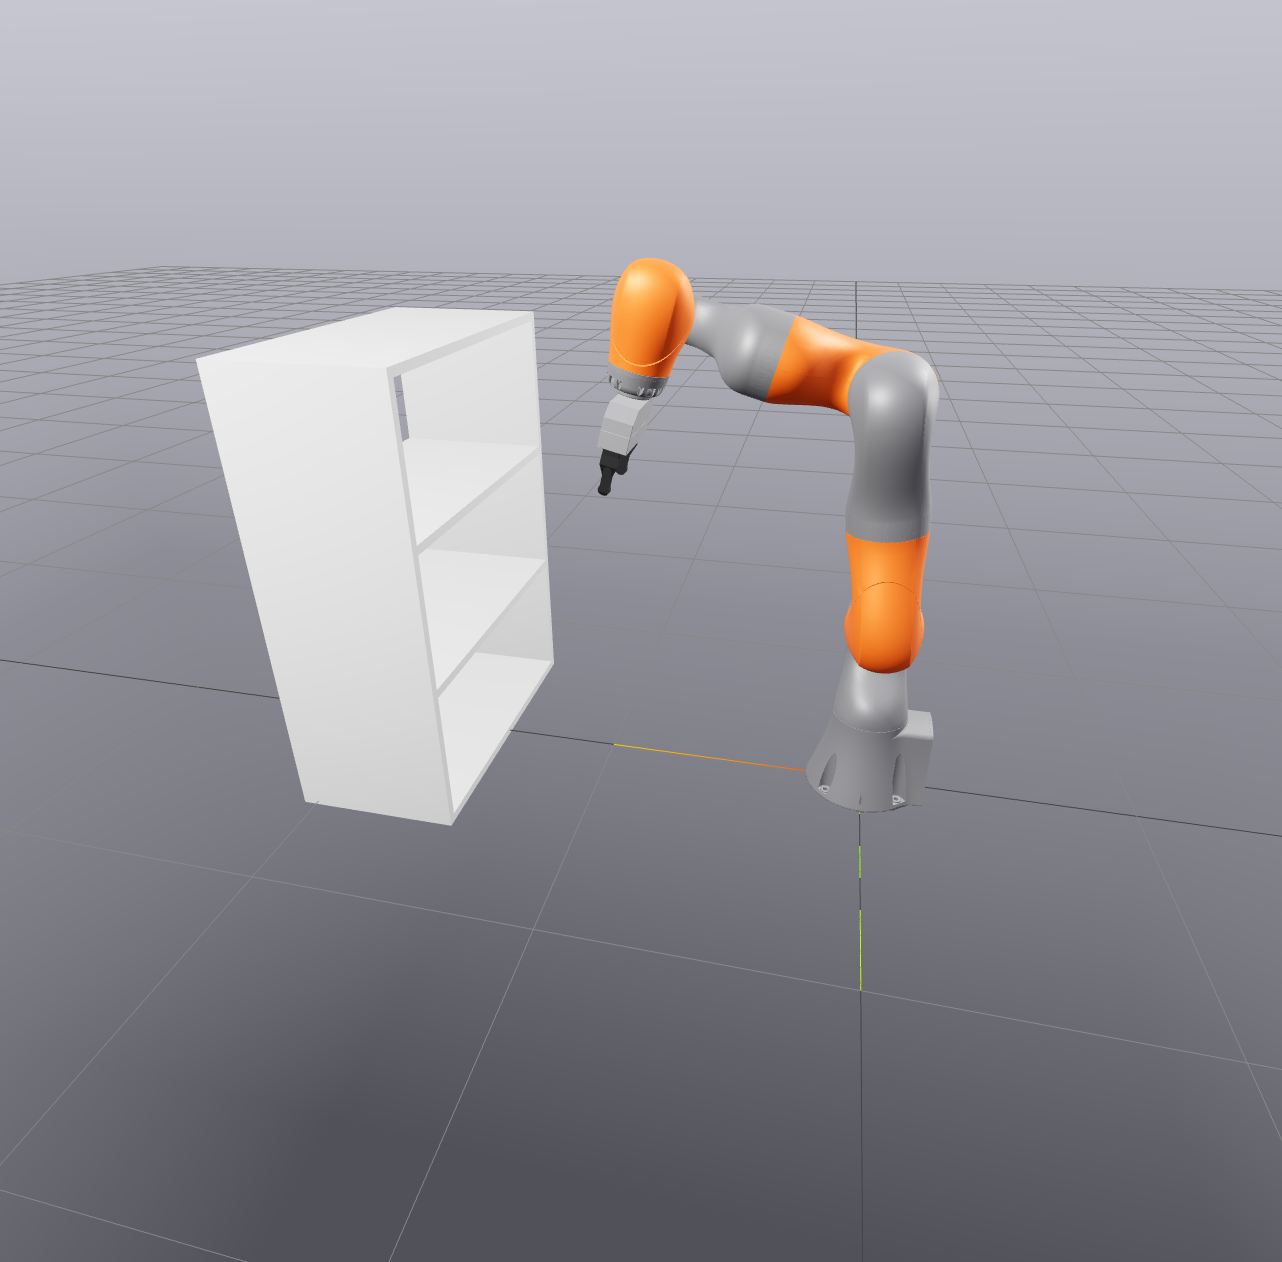
\includegraphics[
            height=3.5cm,
            keepaspectratio
        ]{meshcat1.png}
        \caption{Манипулятор и одна полка}
    \end{subfigure}
    \hfill
    \begin{subfigure}[t]{0.32\textwidth}
        \centering
        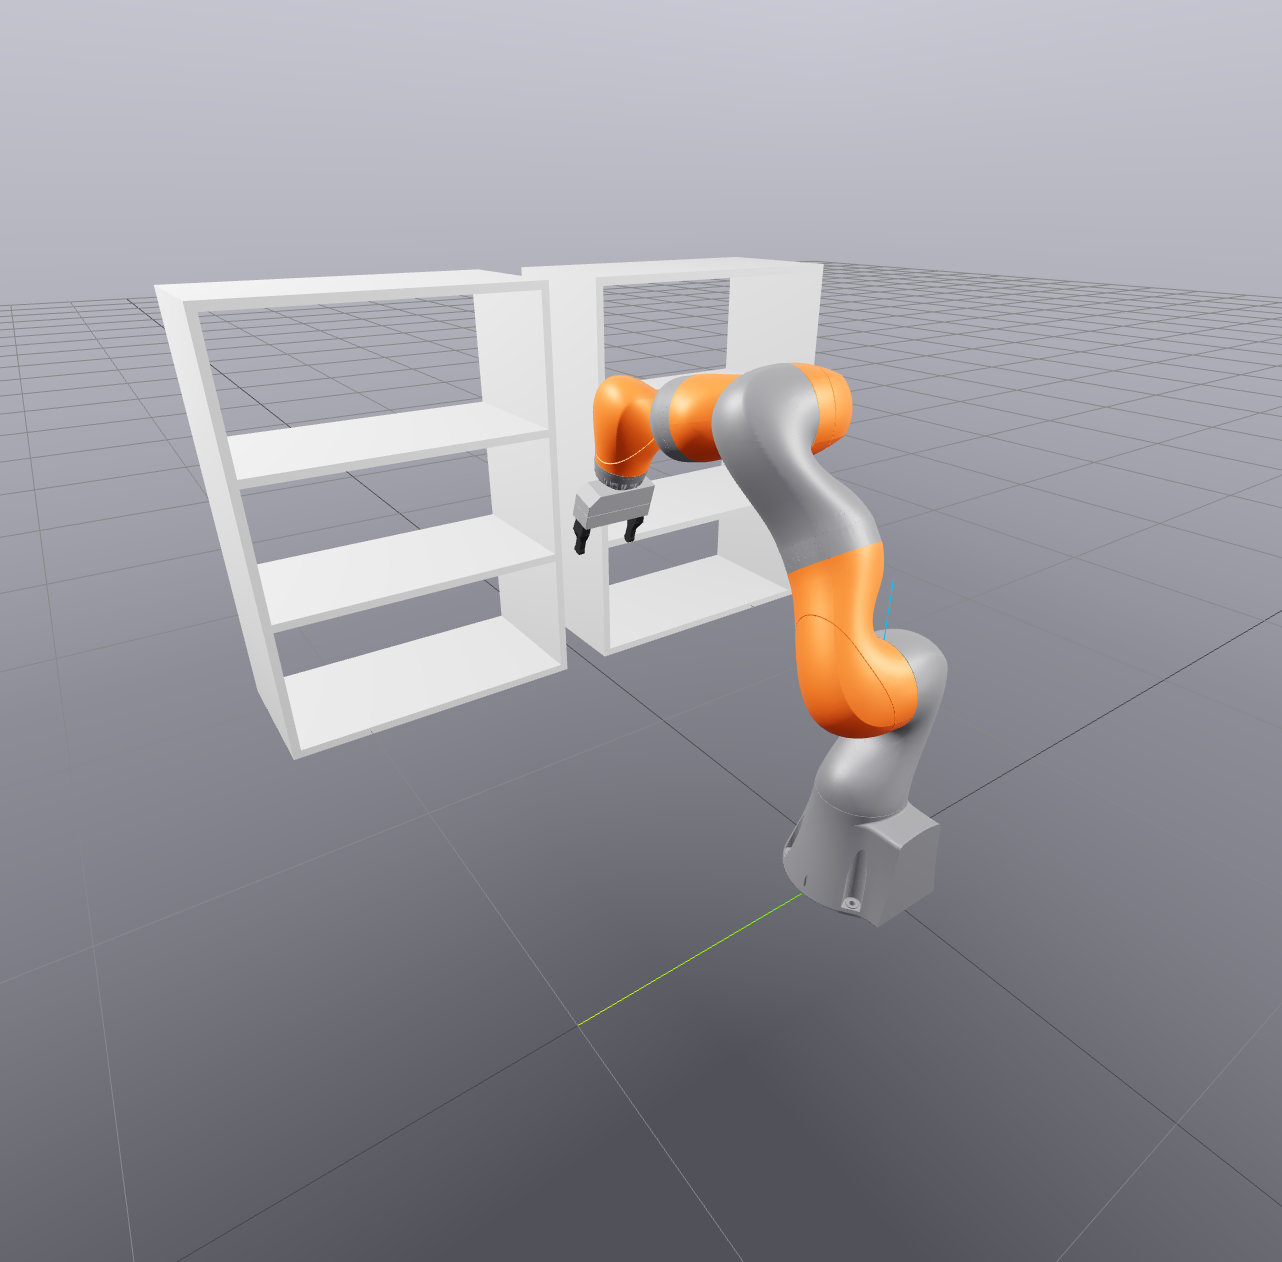
\includegraphics[
            height=3.5cm,
            keepaspectratio
        ]{meshcat2.png}
        \caption{Манипулятор и две параллельные полки}
    \end{subfigure}
    \hfill
    \begin{subfigure}[t]{0.32\textwidth}
        \centering
        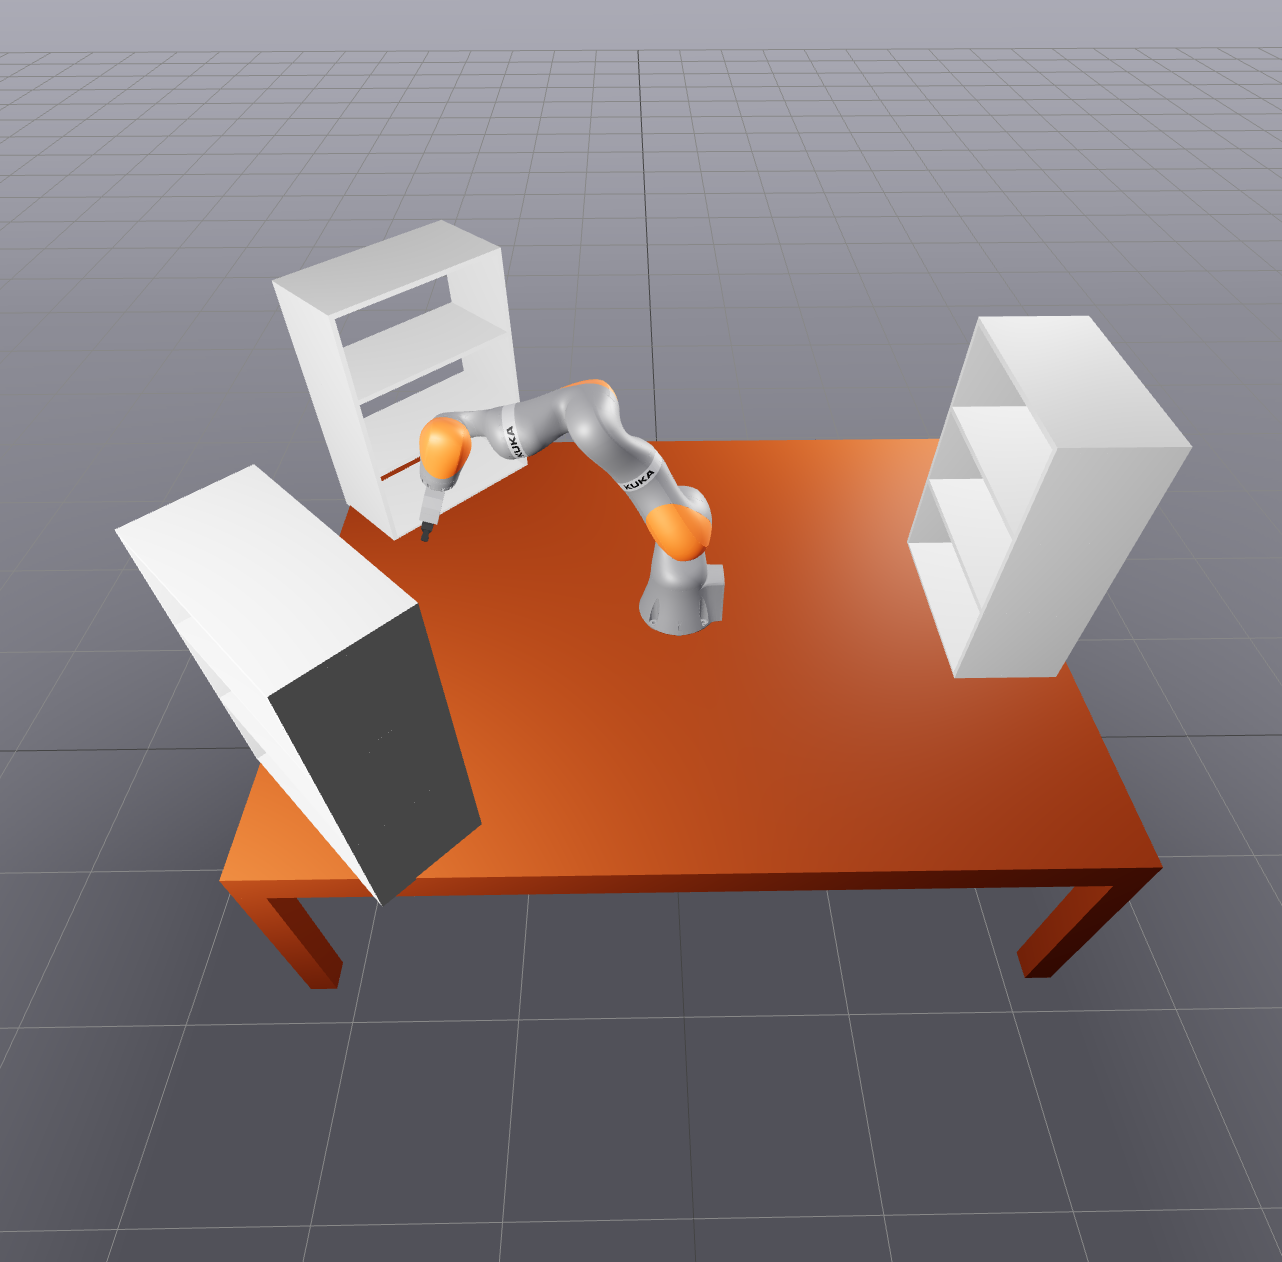
\includegraphics[
            height=3.5cm,
            keepaspectratio
        ]{meshcat3.png}
        \caption{Манипулятор и три полки вокруг него}
    \end{subfigure}

    \caption{Экспериментальные сцены, использованные для построения IRIS-регионов}
    \label{fig:scenes}
\end{figure}



\section{Построение экспериментов}
Для каждой сцены было выполнено по два независимых запуска экспериментов с генерацией 10, 20, 30 и 50 начальных точек для алгоритма IRIS, что в сумме составило 24 эксперимента.
В каждом запуске измерялись время построения выпуклых регионов, количество изолированных (не пересекающихся с другими) выпуклых регионов, а также покрытие сцены.
Оценка покрытия выполнялась с использованием метода Монте-Карло на основе 200 случайных collision-free конфигураций в конфигурационном пространстве манипулятора,
сгенерированных независимо от seed-точек IRIS; покрытие определялось как доля тестовых конфигураций, попавших хотя бы в один выпуклый регион. Следует отметить,
что такая оценка является приближённой, 
и может быть чувствительна к неравномерному распределению выпуклых регионов.

\begin{figure}[h!]
    \centering
    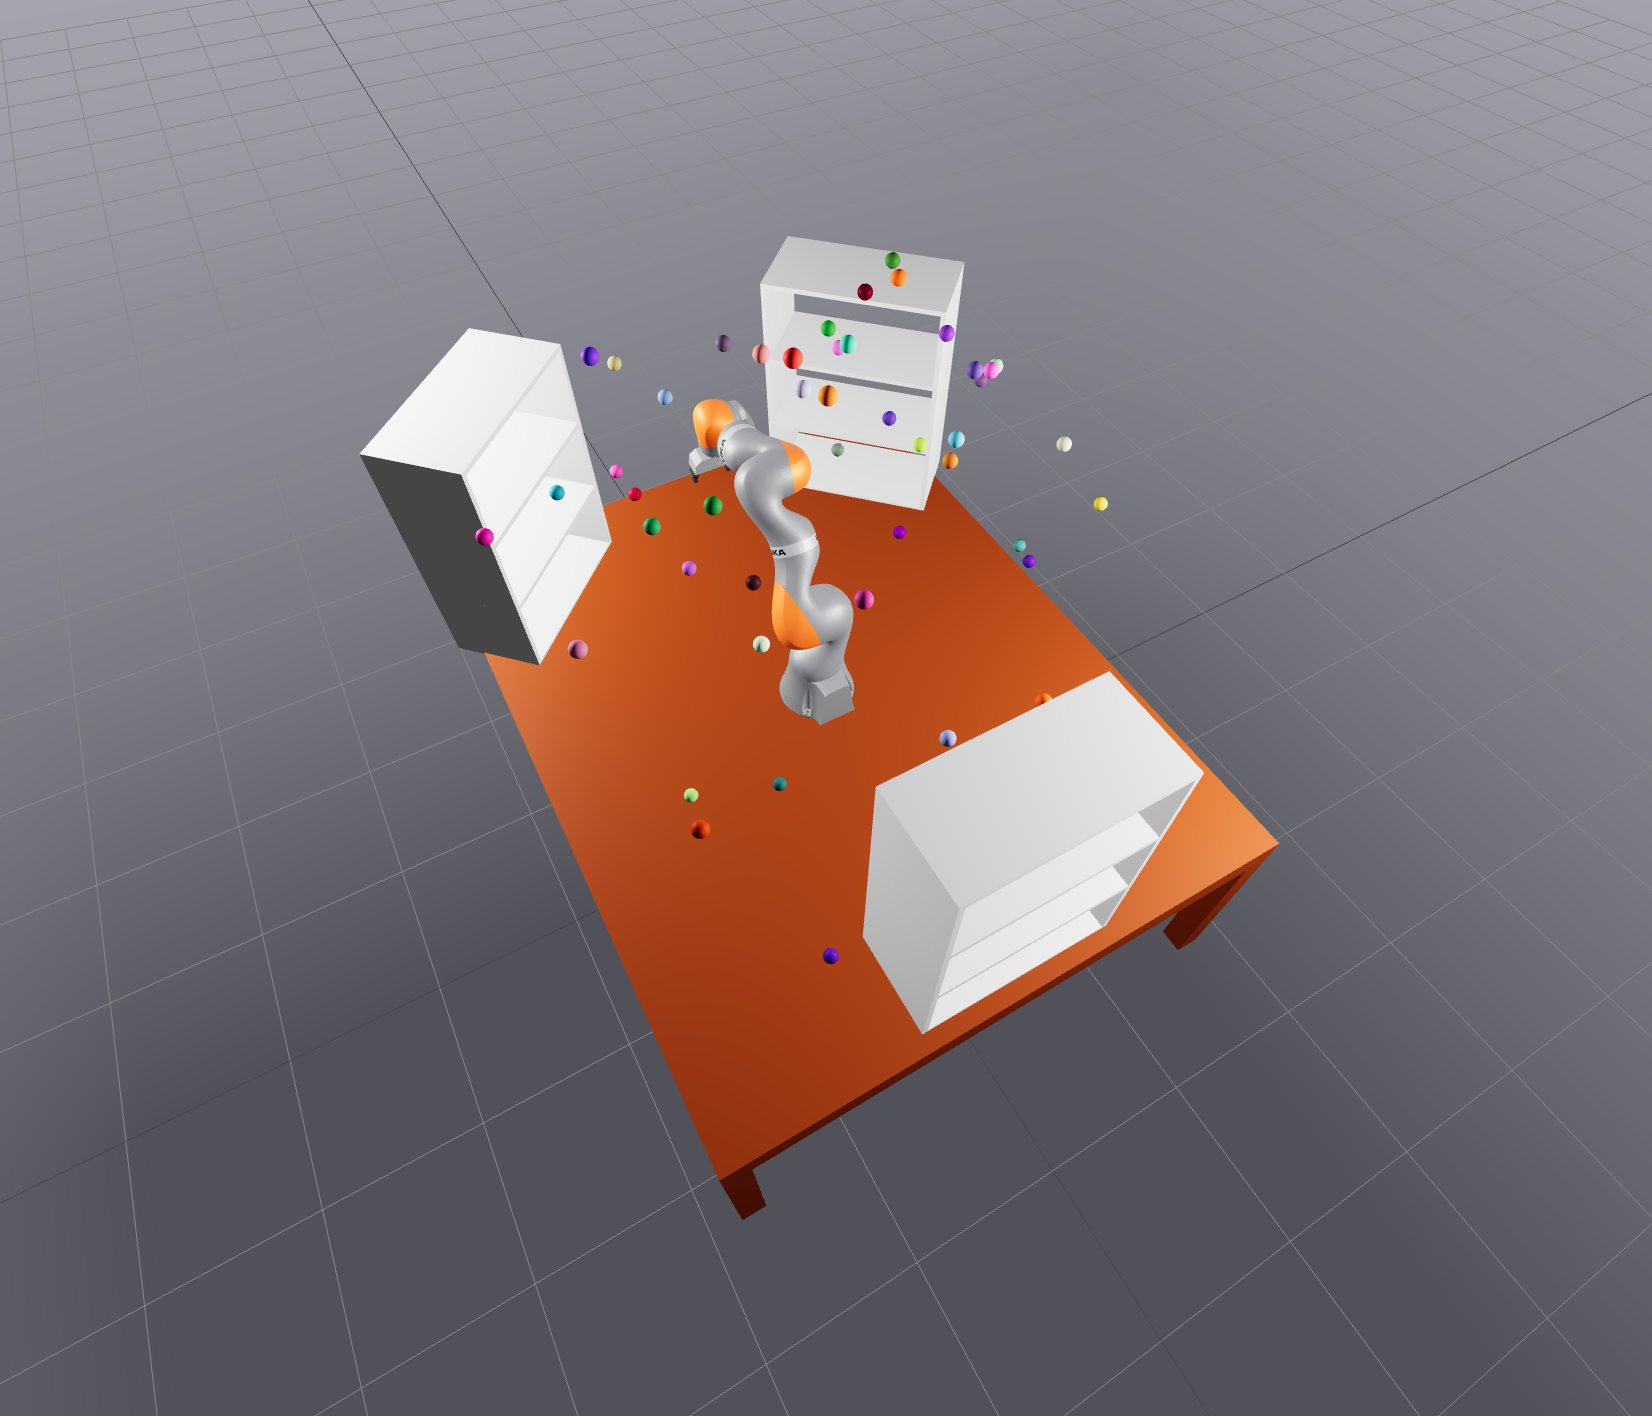
\includegraphics[
        height=6.1cm,
        keepaspectratio
    ]{meshcat_points.png}
    \caption{Случайно сгенерированные начальные точки для алгоритма IRIS}
    \label{fig:iris-seeds}
\end{figure}
\section{Результаты экспериментов и анализ}
Результаты экспериментов приведены в таблице. Ожидаемо самое хорошее покрытие получали эксперименты с большим количеством начальных точек. Однако, для 50 точек время построения выпуклых регионов достигает 1299 секунд в случае сцены с тремя полками, что достаточно много. 
Более того, как видно из таблицы, чем сложнее сцена, тем больше необходимо точек для ее покрытия, а значит построение выпуклых регионов при произвольных начальных точках будет работать дольше с возрастанием сложности сцены. Так же стоит отметить, что выпуклые регионы на произвольных точках плохо покрывают узкие места сцены.
Наример, в нашем случае некоторые полки на сцене остались частично не покрытыми выпуклыми регионами. 
\begin{table}[H]
\centering
\caption{IRIS Coverage Analysis across scenes and number of seed points.}
\label{tab:iris_coverage}
\begin{tabular}{l
                S[table-format=2.0]
                S[table-format=2.1]
                S[table-format=1.1]
                S[table-format=2.0]
                S[table-format=2.1]
                S[table-format=4.0]}
\toprule
\textbf{Scene} & \textbf{Seeds} & \textbf{Regions} & \textbf{Isolation\%} & \textbf{Coverage\%} & \textbf{IRIS Time (s)} \\
\midrule
SINGLE\_SHELF          & 10 & 10.0 & 0.0 & 67.0 \pm 2.8 & 63  \\
SINGLE\_SHELF          & 20 & 20.0 & 0.0 & 67.8 \pm 3.9 & 156 \\
SINGLE\_SHELF          & 30 & 30.0 & 0.0 & 76.2 \pm 5.3 & 180 \\
SINGLE\_SHELF          & 50 & 50.0 & 0.0 & 83.0 \pm 2.1 & 319 \\
\addlinespace
TABLE\_THREE\_SHELVES  & 10 &  9.0 & 0.0 & 40.2 \pm 0.4 & 348 \\
TABLE\_THREE\_SHELVES  & 20 & 19.5 & 0.0 & 47.2 \pm 5.3 & 413 \\
TABLE\_THREE\_SHELVES  & 30 & 29.5 & 0.5 \pm 0.7 & 51.5 \pm 2.1 & 691 \\
TABLE\_THREE\_SHELVES  & 50 & 49.5 & 0.5 \pm 0.7 & 60.2 \pm 5.3 & 1299 \\
\addlinespace
TWO\_SHELVES           & 10 & 10.0 & 0.0 & 66.3 \pm 3.2 & 97  \\
TWO\_SHELVES           & 20 & 20.0 & 0.0 & 72.2 \pm 1.8 & 218 \\
TWO\_SHELVES           & 30 & 29.5 & 0.0 & 75.2 \pm 2.5 & 256 \\
TWO\_SHELVES           & 50 & 50.0 & 0.0 & 82.2 \pm 1.8 & 430 \\
\bottomrule
\end{tabular}
\end{table}


\section{Дальнейшее направление работы}

\end{document}